%!TEX root = main.tex
\setcounter{chapter}{6}
\setcounter{section}{5}
\setcounter{theorem}{0}
\setcounter{equation}{0}

\lectureheader{161}{Calculus I}{Work and fluid forces}{\textit{Thomas' Calculus} \thesection}


\begin{definition}
The \textbf{work} done by a \underline{constant} force $F$ on an object as it is displaced $d$ units in a \underline{straight line} in the same or opposite direction of the force is $W = Fd$.
\end{definition}

\begin{example}
A 5-\si{kg} bucket is lifted from the ground into the air by pulling in 20 \si{m} of rope at a constant speed.
If the linear density of the rope is $\delta=0.08$ \si{kg/m}, how much work is done in lifting the bucket and rope?
\end{example}
\begin{flushright}
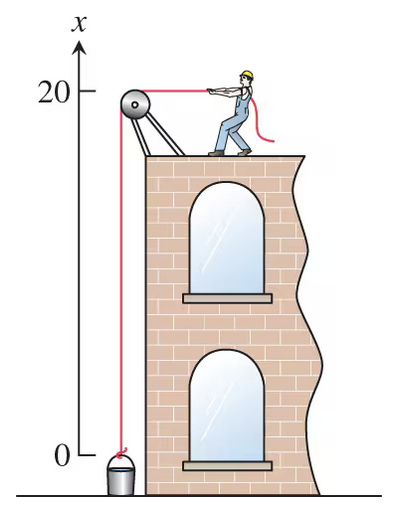
\includegraphics[width=2in]{img/work_on_rope}
\end{flushright}

\ifdefined\SOLUTION
\SOLUTION{
To lift the bucket and rope at a constant speed, the force $F$ applied by the worker must equal the force due to gravity.
Thus lifting the 5-\si{kg} bucket 20 meters into the air simply requires
\begin{equation*}
W_0 = 5\cdot g\cdot 20 = 100g = 980
\end{equation*}
\si{N\cdot m} or Joules.
However, the 20 meters of rope also has mass, and so it requires work to lift the rope along with the bucket.
This is not a simple problem since not all of the rope has to be lifted the full 20 meters.
To address this problem, we let $x$ measure the distance from the ground (in meters), 
and we slice the rope into ``infinitesimal pieces" of length $\dee x$ meters.
Gravity exerts a force of $-g\cdot c\dee x$ Newtons on such a slice of rope.
Thus, the worker must exert a force of 
\begin{equation*}
F=g\cdot c\dee x
\end{equation*}
Netwons to lift this slice at a constant speed,
and the slice at position $x$ must be lifted $(20-x)$ meters.
Therefore, the work to lift the full 20 meters of rope is
\begin{equation*}
W_1 = \int_0^{20}gc(20-x)\dee x = gc\left(20x -\frac{x^2}{2}\right)\Big|_0^{20} = 156.8
\end{equation*}
Joules so that the total work to lift the rope and bucket is
\begin{equation*}
W = W_0 + W_1 = 1136.8
\end{equation*}
Joules.
}
\fi

\newpage

\begin{example}
A tank has the shape of an inverted circular cone of height 10 \si{ft} and base radius 5 \si{ft}.
Suppose the tank is filled to within 2 \si{ft} of the top with olive oil weighing 57 \si{lb/ft^3}.
How much work does it take to pump the oid to the rim of the tank?
\end{example}
\begin{flushright}
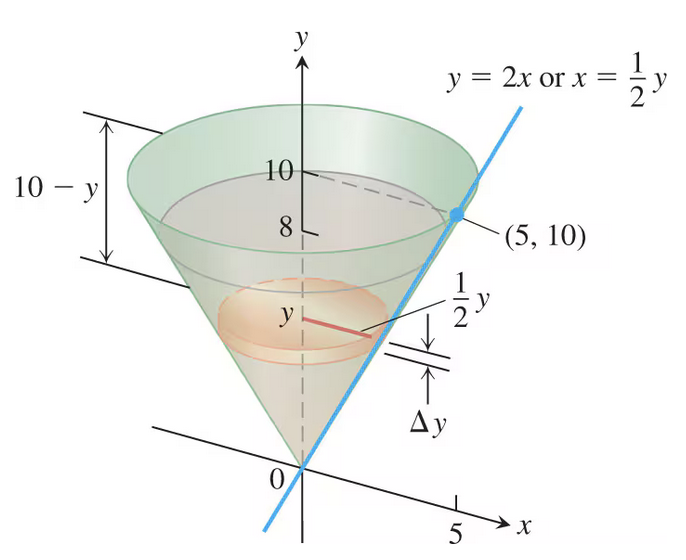
\includegraphics[width=3in]{img/work_by_pump}
\end{flushright}

\newpage

\begin{definition}
\textbf{Pressure} is the amount of force per unit area applied perpendicularly to the surface of an object.
\end{definition}

\begin{remark}
When an object is submerged in a fluid, the pressure at any point on its surface depends on the depth.
In a standing fluid of weight-density $w$, the pressure at depth $h$ is
\begin{equation*}
P = wh.
\end{equation*}
\end{remark}

\begin{example}
A dam has the shape of an isosceles trapezoid.
The height of the dam is 20 \si{m}, the width at the top is 50 \si{m}, and the width at the bottom is 30 \si{m}.
Find the total force due to hydrostatic pressure if the water level is 4 \si{m} from the top of the dam, assuming that the mass-density of water is $\delta = 1000$ \si{kg/m^3}.
\end{example}

\ifdefined\SOLUTION
\SOLUTION{
First we observe that the weight-density of water is 
\begin{equation*}
w = \delta g = 1000\cdot 9.8 = 9800\ \si{N/m^3}.
\end{equation*}
Note that 1 \si{N} = 1 \si{kg\cdot m/s^2}.
}
\fi
